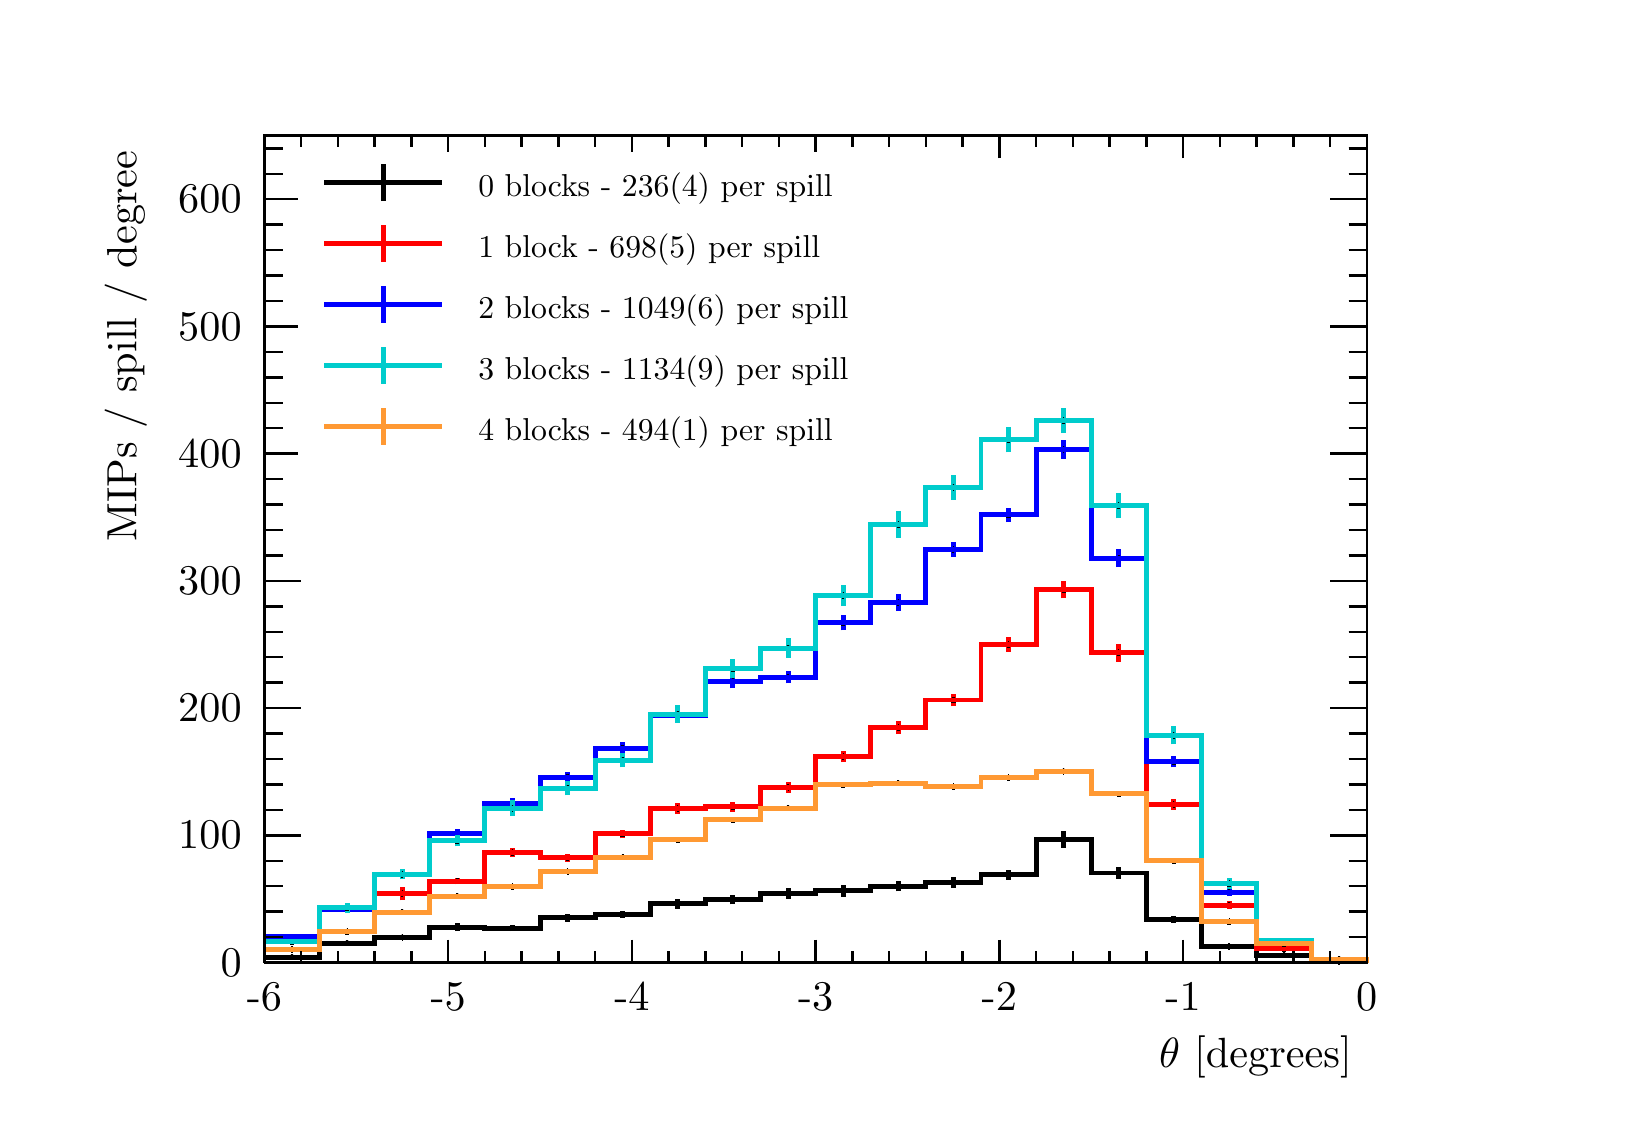
\begin{tikzpicture}
\pgfdeclareplotmark{cross} {
\pgfpathmoveto{\pgfpoint{-0.3\pgfplotmarksize}{\pgfplotmarksize}}
\pgfpathlineto{\pgfpoint{+0.3\pgfplotmarksize}{\pgfplotmarksize}}
\pgfpathlineto{\pgfpoint{+0.3\pgfplotmarksize}{0.3\pgfplotmarksize}}
\pgfpathlineto{\pgfpoint{+1\pgfplotmarksize}{0.3\pgfplotmarksize}}
\pgfpathlineto{\pgfpoint{+1\pgfplotmarksize}{-0.3\pgfplotmarksize}}
\pgfpathlineto{\pgfpoint{+0.3\pgfplotmarksize}{-0.3\pgfplotmarksize}}
\pgfpathlineto{\pgfpoint{+0.3\pgfplotmarksize}{-1.\pgfplotmarksize}}
\pgfpathlineto{\pgfpoint{-0.3\pgfplotmarksize}{-1.\pgfplotmarksize}}
\pgfpathlineto{\pgfpoint{-0.3\pgfplotmarksize}{-0.3\pgfplotmarksize}}
\pgfpathlineto{\pgfpoint{-1.\pgfplotmarksize}{-0.3\pgfplotmarksize}}
\pgfpathlineto{\pgfpoint{-1.\pgfplotmarksize}{0.3\pgfplotmarksize}}
\pgfpathlineto{\pgfpoint{-0.3\pgfplotmarksize}{0.3\pgfplotmarksize}}
\pgfpathclose
\pgfusepathqstroke
}
\pgfdeclareplotmark{cross*} {
\pgfpathmoveto{\pgfpoint{-0.3\pgfplotmarksize}{\pgfplotmarksize}}
\pgfpathlineto{\pgfpoint{+0.3\pgfplotmarksize}{\pgfplotmarksize}}
\pgfpathlineto{\pgfpoint{+0.3\pgfplotmarksize}{0.3\pgfplotmarksize}}
\pgfpathlineto{\pgfpoint{+1\pgfplotmarksize}{0.3\pgfplotmarksize}}
\pgfpathlineto{\pgfpoint{+1\pgfplotmarksize}{-0.3\pgfplotmarksize}}
\pgfpathlineto{\pgfpoint{+0.3\pgfplotmarksize}{-0.3\pgfplotmarksize}}
\pgfpathlineto{\pgfpoint{+0.3\pgfplotmarksize}{-1.\pgfplotmarksize}}
\pgfpathlineto{\pgfpoint{-0.3\pgfplotmarksize}{-1.\pgfplotmarksize}}
\pgfpathlineto{\pgfpoint{-0.3\pgfplotmarksize}{-0.3\pgfplotmarksize}}
\pgfpathlineto{\pgfpoint{-1.\pgfplotmarksize}{-0.3\pgfplotmarksize}}
\pgfpathlineto{\pgfpoint{-1.\pgfplotmarksize}{0.3\pgfplotmarksize}}
\pgfpathlineto{\pgfpoint{-0.3\pgfplotmarksize}{0.3\pgfplotmarksize}}
\pgfpathclose
\pgfusepathqfillstroke
}
\pgfdeclareplotmark{newstar} {
\pgfpathmoveto{\pgfqpoint{0pt}{\pgfplotmarksize}}
\pgfpathlineto{\pgfqpointpolar{44}{0.5\pgfplotmarksize}}
\pgfpathlineto{\pgfqpointpolar{18}{\pgfplotmarksize}}
\pgfpathlineto{\pgfqpointpolar{-20}{0.5\pgfplotmarksize}}
\pgfpathlineto{\pgfqpointpolar{-54}{\pgfplotmarksize}}
\pgfpathlineto{\pgfqpointpolar{-90}{0.5\pgfplotmarksize}}
\pgfpathlineto{\pgfqpointpolar{234}{\pgfplotmarksize}}
\pgfpathlineto{\pgfqpointpolar{198}{0.5\pgfplotmarksize}}
\pgfpathlineto{\pgfqpointpolar{162}{\pgfplotmarksize}}
\pgfpathlineto{\pgfqpointpolar{134}{0.5\pgfplotmarksize}}
\pgfpathclose
\pgfusepathqstroke
}
\pgfdeclareplotmark{newstar*} {
\pgfpathmoveto{\pgfqpoint{0pt}{\pgfplotmarksize}}
\pgfpathlineto{\pgfqpointpolar{44}{0.5\pgfplotmarksize}}
\pgfpathlineto{\pgfqpointpolar{18}{\pgfplotmarksize}}
\pgfpathlineto{\pgfqpointpolar{-20}{0.5\pgfplotmarksize}}
\pgfpathlineto{\pgfqpointpolar{-54}{\pgfplotmarksize}}
\pgfpathlineto{\pgfqpointpolar{-90}{0.5\pgfplotmarksize}}
\pgfpathlineto{\pgfqpointpolar{234}{\pgfplotmarksize}}
\pgfpathlineto{\pgfqpointpolar{198}{0.5\pgfplotmarksize}}
\pgfpathlineto{\pgfqpointpolar{162}{\pgfplotmarksize}}
\pgfpathlineto{\pgfqpointpolar{134}{0.5\pgfplotmarksize}}
\pgfpathclose
\pgfusepathqfillstroke
}
\definecolor{c}{rgb}{1,1,1};
\draw [color=c, fill=c] (0,0) rectangle (20,13.639);
\draw [color=c, fill=c] (3,1.77307) rectangle (17,12.2751);
\definecolor{c}{rgb}{0,0,0};
\draw [c,line width=0.9] (3,1.77307) -- (3,12.2751) -- (17,12.2751) -- (17,1.77307) -- (3,1.77307);
\definecolor{c}{rgb}{1,1,1};
\draw [color=c, fill=c] (3,1.77307) rectangle (17,12.2751);
\definecolor{c}{rgb}{0,0,0};
\draw [c,line width=0.9] (3,1.77307) -- (3,12.2751) -- (17,12.2751) -- (17,1.77307) -- (3,1.77307);
\draw [c,line width=0.9] (3,1.77307) -- (3.7,1.77307) -- (3.7,1.77307) -- (4.4,1.77307) -- (4.4,1.77307) -- (5.1,1.77307) -- (5.1,1.77307) -- (5.8,1.77307) -- (5.8,1.77307) -- (6.5,1.77307) -- (6.5,1.77307) -- (7.2,1.77307) -- (7.2,1.77307) --
 (7.9,1.77307) -- (7.9,1.77307) -- (8.6,1.77307) -- (8.6,1.77307) -- (9.3,1.77307) -- (9.3,1.77307) -- (10,1.77307) -- (10,1.77307) -- (10.7,1.77307) -- (10.7,1.77307) -- (11.4,1.77307) -- (11.4,1.77307) -- (12.1,1.77307) -- (12.1,1.77307) --
 (12.8,1.77307) -- (12.8,1.77307) -- (13.5,1.77307) -- (13.5,1.77307) -- (14.2,1.77307) -- (14.2,1.77307) -- (14.9,1.77307) -- (14.9,1.77307) -- (15.6,1.77307) -- (15.6,1.77307) -- (16.3,1.77307) -- (16.3,1.77307) -- (17,1.77307) -- (17,1.77307);
\draw [c,line width=0.9] (3,1.77307) -- (17,1.77307);
\draw [c,line width=0.9] (3,2.05948) -- (3,1.77307);
\draw [c,line width=0.9] (3.46667,1.91628) -- (3.46667,1.77307);
\draw [c,line width=0.9] (3.93333,1.91628) -- (3.93333,1.77307);
\draw [c,line width=0.9] (4.4,1.91628) -- (4.4,1.77307);
\draw [c,line width=0.9] (4.86667,1.91628) -- (4.86667,1.77307);
\draw [c,line width=0.9] (5.33333,2.05948) -- (5.33333,1.77307);
\draw [c,line width=0.9] (5.8,1.91628) -- (5.8,1.77307);
\draw [c,line width=0.9] (6.26667,1.91628) -- (6.26667,1.77307);
\draw [c,line width=0.9] (6.73333,1.91628) -- (6.73333,1.77307);
\draw [c,line width=0.9] (7.2,1.91628) -- (7.2,1.77307);
\draw [c,line width=0.9] (7.66667,2.05948) -- (7.66667,1.77307);
\draw [c,line width=0.9] (8.13333,1.91628) -- (8.13333,1.77307);
\draw [c,line width=0.9] (8.6,1.91628) -- (8.6,1.77307);
\draw [c,line width=0.9] (9.06667,1.91628) -- (9.06667,1.77307);
\draw [c,line width=0.9] (9.53333,1.91628) -- (9.53333,1.77307);
\draw [c,line width=0.9] (10,2.05948) -- (10,1.77307);
\draw [c,line width=0.9] (10.4667,1.91628) -- (10.4667,1.77307);
\draw [c,line width=0.9] (10.9333,1.91628) -- (10.9333,1.77307);
\draw [c,line width=0.9] (11.4,1.91628) -- (11.4,1.77307);
\draw [c,line width=0.9] (11.8667,1.91628) -- (11.8667,1.77307);
\draw [c,line width=0.9] (12.3333,2.05948) -- (12.3333,1.77307);
\draw [c,line width=0.9] (12.8,1.91628) -- (12.8,1.77307);
\draw [c,line width=0.9] (13.2667,1.91628) -- (13.2667,1.77307);
\draw [c,line width=0.9] (13.7333,1.91628) -- (13.7333,1.77307);
\draw [c,line width=0.9] (14.2,1.91628) -- (14.2,1.77307);
\draw [c,line width=0.9] (14.6667,2.05948) -- (14.6667,1.77307);
\draw [c,line width=0.9] (15.1333,1.91628) -- (15.1333,1.77307);
\draw [c,line width=0.9] (15.6,1.91628) -- (15.6,1.77307);
\draw [c,line width=0.9] (16.0667,1.91628) -- (16.0667,1.77307);
\draw [c,line width=0.9] (16.5333,1.91628) -- (16.5333,1.77307);
\draw [c,line width=0.9] (17,2.05948) -- (17,1.77307);
\draw [anchor=base] (3,1.15931) node[scale=1.52731, color=c, rotate=0]{-6};
\draw [anchor=base] (5.33333,1.15931) node[scale=1.52731, color=c, rotate=0]{-5};
\draw [anchor=base] (7.66667,1.15931) node[scale=1.52731, color=c, rotate=0]{-4};
\draw [anchor=base] (10,1.15931) node[scale=1.52731, color=c, rotate=0]{-3};
\draw [anchor=base] (12.3333,1.15931) node[scale=1.52731, color=c, rotate=0]{-2};
\draw [anchor=base] (14.6667,1.15931) node[scale=1.52731, color=c, rotate=0]{-1};
\draw [anchor=base] (17,1.15931) node[scale=1.52731, color=c, rotate=0]{0};
\draw [anchor= east] (17,0.572837) node[scale=1.52731, color=c, rotate=0]{$\theta$ [degrees] };
\draw [c,line width=0.9] (3,12.2751) -- (17,12.2751);
\draw [c,line width=0.9] (3,11.9887) -- (3,12.2751);
\draw [c,line width=0.9] (3.46667,12.1319) -- (3.46667,12.2751);
\draw [c,line width=0.9] (3.93333,12.1319) -- (3.93333,12.2751);
\draw [c,line width=0.9] (4.4,12.1319) -- (4.4,12.2751);
\draw [c,line width=0.9] (4.86667,12.1319) -- (4.86667,12.2751);
\draw [c,line width=0.9] (5.33333,11.9887) -- (5.33333,12.2751);
\draw [c,line width=0.9] (5.8,12.1319) -- (5.8,12.2751);
\draw [c,line width=0.9] (6.26667,12.1319) -- (6.26667,12.2751);
\draw [c,line width=0.9] (6.73333,12.1319) -- (6.73333,12.2751);
\draw [c,line width=0.9] (7.2,12.1319) -- (7.2,12.2751);
\draw [c,line width=0.9] (7.66667,11.9887) -- (7.66667,12.2751);
\draw [c,line width=0.9] (8.13333,12.1319) -- (8.13333,12.2751);
\draw [c,line width=0.9] (8.6,12.1319) -- (8.6,12.2751);
\draw [c,line width=0.9] (9.06667,12.1319) -- (9.06667,12.2751);
\draw [c,line width=0.9] (9.53333,12.1319) -- (9.53333,12.2751);
\draw [c,line width=0.9] (10,11.9887) -- (10,12.2751);
\draw [c,line width=0.9] (10.4667,12.1319) -- (10.4667,12.2751);
\draw [c,line width=0.9] (10.9333,12.1319) -- (10.9333,12.2751);
\draw [c,line width=0.9] (11.4,12.1319) -- (11.4,12.2751);
\draw [c,line width=0.9] (11.8667,12.1319) -- (11.8667,12.2751);
\draw [c,line width=0.9] (12.3333,11.9887) -- (12.3333,12.2751);
\draw [c,line width=0.9] (12.8,12.1319) -- (12.8,12.2751);
\draw [c,line width=0.9] (13.2667,12.1319) -- (13.2667,12.2751);
\draw [c,line width=0.9] (13.7333,12.1319) -- (13.7333,12.2751);
\draw [c,line width=0.9] (14.2,12.1319) -- (14.2,12.2751);
\draw [c,line width=0.9] (14.6667,11.9887) -- (14.6667,12.2751);
\draw [c,line width=0.9] (15.1333,12.1319) -- (15.1333,12.2751);
\draw [c,line width=0.9] (15.6,12.1319) -- (15.6,12.2751);
\draw [c,line width=0.9] (16.0667,12.1319) -- (16.0667,12.2751);
\draw [c,line width=0.9] (16.5333,12.1319) -- (16.5333,12.2751);
\draw [c,line width=0.9] (17,11.9887) -- (17,12.2751);
\draw [c,line width=0.9] (3,1.77307) -- (3,12.2751);
\draw [c,line width=0.9] (3.462,1.77307) -- (3,1.77307);
\draw [c,line width=0.9] (3.231,2.0962) -- (3,2.0962);
\draw [c,line width=0.9] (3.231,2.41934) -- (3,2.41934);
\draw [c,line width=0.9] (3.231,2.74248) -- (3,2.74248);
\draw [c,line width=0.9] (3.231,3.06562) -- (3,3.06562);
\draw [c,line width=0.9] (3.462,3.38876) -- (3,3.38876);
\draw [c,line width=0.9] (3.231,3.7119) -- (3,3.7119);
\draw [c,line width=0.9] (3.231,4.03504) -- (3,4.03504);
\draw [c,line width=0.9] (3.231,4.35817) -- (3,4.35817);
\draw [c,line width=0.9] (3.231,4.68131) -- (3,4.68131);
\draw [c,line width=0.9] (3.462,5.00445) -- (3,5.00445);
\draw [c,line width=0.9] (3.231,5.32759) -- (3,5.32759);
\draw [c,line width=0.9] (3.231,5.65073) -- (3,5.65073);
\draw [c,line width=0.9] (3.231,5.97387) -- (3,5.97387);
\draw [c,line width=0.9] (3.231,6.29701) -- (3,6.29701);
\draw [c,line width=0.9] (3.462,6.62015) -- (3,6.62015);
\draw [c,line width=0.9] (3.231,6.94328) -- (3,6.94328);
\draw [c,line width=0.9] (3.231,7.26642) -- (3,7.26642);
\draw [c,line width=0.9] (3.231,7.58956) -- (3,7.58956);
\draw [c,line width=0.9] (3.231,7.9127) -- (3,7.9127);
\draw [c,line width=0.9] (3.462,8.23584) -- (3,8.23584);
\draw [c,line width=0.9] (3.231,8.55898) -- (3,8.55898);
\draw [c,line width=0.9] (3.231,8.88212) -- (3,8.88212);
\draw [c,line width=0.9] (3.231,9.20525) -- (3,9.20525);
\draw [c,line width=0.9] (3.231,9.52839) -- (3,9.52839);
\draw [c,line width=0.9] (3.462,9.85153) -- (3,9.85153);
\draw [c,line width=0.9] (3.231,10.1747) -- (3,10.1747);
\draw [c,line width=0.9] (3.231,10.4978) -- (3,10.4978);
\draw [c,line width=0.9] (3.231,10.8209) -- (3,10.8209);
\draw [c,line width=0.9] (3.231,11.1441) -- (3,11.1441);
\draw [c,line width=0.9] (3.462,11.4672) -- (3,11.4672);
\draw [c,line width=0.9] (3.462,11.4672) -- (3,11.4672);
\draw [c,line width=0.9] (3.231,11.7904) -- (3,11.7904);
\draw [c,line width=0.9] (3.231,12.1135) -- (3,12.1135);
\draw [anchor= east] (2.9,1.77307) node[scale=1.52731, color=c, rotate=0]{0};
\draw [anchor= east] (2.9,3.38876) node[scale=1.52731, color=c, rotate=0]{100};
\draw [anchor= east] (2.9,5.00445) node[scale=1.52731, color=c, rotate=0]{200};
\draw [anchor= east] (2.9,6.62015) node[scale=1.52731, color=c, rotate=0]{300};
\draw [anchor= east] (2.9,8.23584) node[scale=1.52731, color=c, rotate=0]{400};
\draw [anchor= east] (2.9,9.85153) node[scale=1.52731, color=c, rotate=0]{500};
\draw [anchor= east] (2.9,11.4672) node[scale=1.52731, color=c, rotate=0]{600};
\draw [anchor= east] (1.24,12.2751) node[scale=1.52731, color=c, rotate=90]{ MIPs / spill / degree};
\draw [c,line width=0.9] (17,1.77307) -- (17,12.2751);
\draw [c,line width=0.9] (16.538,1.77307) -- (17,1.77307);
\draw [c,line width=0.9] (16.769,2.0962) -- (17,2.0962);
\draw [c,line width=0.9] (16.769,2.41934) -- (17,2.41934);
\draw [c,line width=0.9] (16.769,2.74248) -- (17,2.74248);
\draw [c,line width=0.9] (16.769,3.06562) -- (17,3.06562);
\draw [c,line width=0.9] (16.538,3.38876) -- (17,3.38876);
\draw [c,line width=0.9] (16.769,3.7119) -- (17,3.7119);
\draw [c,line width=0.9] (16.769,4.03504) -- (17,4.03504);
\draw [c,line width=0.9] (16.769,4.35817) -- (17,4.35817);
\draw [c,line width=0.9] (16.769,4.68131) -- (17,4.68131);
\draw [c,line width=0.9] (16.538,5.00445) -- (17,5.00445);
\draw [c,line width=0.9] (16.769,5.32759) -- (17,5.32759);
\draw [c,line width=0.9] (16.769,5.65073) -- (17,5.65073);
\draw [c,line width=0.9] (16.769,5.97387) -- (17,5.97387);
\draw [c,line width=0.9] (16.769,6.29701) -- (17,6.29701);
\draw [c,line width=0.9] (16.538,6.62015) -- (17,6.62015);
\draw [c,line width=0.9] (16.769,6.94328) -- (17,6.94328);
\draw [c,line width=0.9] (16.769,7.26642) -- (17,7.26642);
\draw [c,line width=0.9] (16.769,7.58956) -- (17,7.58956);
\draw [c,line width=0.9] (16.769,7.9127) -- (17,7.9127);
\draw [c,line width=0.9] (16.538,8.23584) -- (17,8.23584);
\draw [c,line width=0.9] (16.769,8.55898) -- (17,8.55898);
\draw [c,line width=0.9] (16.769,8.88212) -- (17,8.88212);
\draw [c,line width=0.9] (16.769,9.20525) -- (17,9.20525);
\draw [c,line width=0.9] (16.769,9.52839) -- (17,9.52839);
\draw [c,line width=0.9] (16.538,9.85153) -- (17,9.85153);
\draw [c,line width=0.9] (16.769,10.1747) -- (17,10.1747);
\draw [c,line width=0.9] (16.769,10.4978) -- (17,10.4978);
\draw [c,line width=0.9] (16.769,10.8209) -- (17,10.8209);
\draw [c,line width=0.9] (16.769,11.1441) -- (17,11.1441);
\draw [c,line width=0.9] (16.538,11.4672) -- (17,11.4672);
\draw [c,line width=0.9] (16.538,11.4672) -- (17,11.4672);
\draw [c,line width=0.9] (16.769,11.7904) -- (17,11.7904);
\draw [c,line width=0.9] (16.769,12.1135) -- (17,12.1135);
\draw [c,line width=1.8] (3.35,1.83523) -- (3.35,1.84254);
\draw [c,line width=1.8] (3.35,1.84254) -- (3.35,1.84986);
\foreach \P in {(3.35,1.84254)}{\draw[mark options={color=c,fill=c},mark size=2.402402pt, line width=0.000000pt, mark=*,mark size=1pt] plot coordinates {\P};}
\draw [c,line width=1.8] (4.05,1.99334) -- (4.05,2.02111);
\draw [c,line width=1.8] (4.05,2.02111) -- (4.05,2.04887);
\foreach \P in {(4.05,2.02111)}{\draw[mark options={color=c,fill=c},mark size=2.402402pt, line width=0.000000pt, mark=*,mark size=1pt] plot coordinates {\P};}
\draw [c,line width=1.8] (4.75,2.0605) -- (4.75,2.09382);
\draw [c,line width=1.8] (4.75,2.09382) -- (4.75,2.12714);
\foreach \P in {(4.75,2.09382)}{\draw[mark options={color=c,fill=c},mark size=2.402402pt, line width=0.000000pt, mark=*,mark size=1pt] plot coordinates {\P};}
\draw [c,line width=1.8] (5.45,2.17228) -- (5.45,2.22258);
\draw [c,line width=1.8] (5.45,2.22258) -- (5.45,2.27288);
\foreach \P in {(5.45,2.22258)}{\draw[mark options={color=c,fill=c},mark size=2.402402pt, line width=0.000000pt, mark=*,mark size=1pt] plot coordinates {\P};}
\draw [c,line width=1.8] (6.15,2.1727) -- (6.15,2.20944);
\draw [c,line width=1.8] (6.15,2.20944) -- (6.15,2.24619);
\foreach \P in {(6.15,2.20944)}{\draw[mark options={color=c,fill=c},mark size=2.402402pt, line width=0.000000pt, mark=*,mark size=1pt] plot coordinates {\P};}
\draw [c,line width=1.8] (6.85,2.29338) -- (6.85,2.34203);
\draw [c,line width=1.8] (6.85,2.34203) -- (6.85,2.39068);
\foreach \P in {(6.85,2.34203)}{\draw[mark options={color=c,fill=c},mark size=2.402402pt, line width=0.000000pt, mark=*,mark size=1pt] plot coordinates {\P};}
\draw [c,line width=1.8] (7.55,2.33582) -- (7.55,2.37902);
\draw [c,line width=1.8] (7.55,2.37902) -- (7.55,2.42223);
\foreach \P in {(7.55,2.37902)}{\draw[mark options={color=c,fill=c},mark size=2.402402pt, line width=0.000000pt, mark=*,mark size=1pt] plot coordinates {\P};}
\draw [c,line width=1.8] (8.25,2.45782) -- (8.25,2.51906);
\draw [c,line width=1.8] (8.25,2.51906) -- (8.25,2.5803);
\foreach \P in {(8.25,2.51906)}{\draw[mark options={color=c,fill=c},mark size=2.402402pt, line width=0.000000pt, mark=*,mark size=1pt] plot coordinates {\P};}
\draw [c,line width=1.8] (8.95,2.5108) -- (8.95,2.56961);
\draw [c,line width=1.8] (8.95,2.56961) -- (8.95,2.62843);
\foreach \P in {(8.95,2.56961)}{\draw[mark options={color=c,fill=c},mark size=2.402402pt, line width=0.000000pt, mark=*,mark size=1pt] plot coordinates {\P};}
\draw [c,line width=1.8] (9.65,2.58548) -- (9.65,2.64957);
\draw [c,line width=1.8] (9.65,2.64957) -- (9.65,2.71366);
\foreach \P in {(9.65,2.64957)}{\draw[mark options={color=c,fill=c},mark size=2.402402pt, line width=0.000000pt, mark=*,mark size=1pt] plot coordinates {\P};}
\draw [c,line width=1.8] (10.35,2.60955) -- (10.35,2.68222);
\draw [c,line width=1.8] (10.35,2.68222) -- (10.35,2.75489);
\foreach \P in {(10.35,2.68222)}{\draw[mark options={color=c,fill=c},mark size=2.402402pt, line width=0.000000pt, mark=*,mark size=1pt] plot coordinates {\P};}
\draw [c,line width=1.8] (11.05,2.67651) -- (11.05,2.73995);
\draw [c,line width=1.8] (11.05,2.73995) -- (11.05,2.8034);
\foreach \P in {(11.05,2.73995)}{\draw[mark options={color=c,fill=c},mark size=2.402402pt, line width=0.000000pt, mark=*,mark size=1pt] plot coordinates {\P};}
\draw [c,line width=1.8] (11.75,2.71902) -- (11.75,2.78951);
\draw [c,line width=1.8] (11.75,2.78951) -- (11.75,2.86);
\foreach \P in {(11.75,2.78951)}{\draw[mark options={color=c,fill=c},mark size=2.402402pt, line width=0.000000pt, mark=*,mark size=1pt] plot coordinates {\P};}
\draw [c,line width=1.8] (12.45,2.8268) -- (12.45,2.88516);
\draw [c,line width=1.8] (12.45,2.88516) -- (12.45,2.94352);
\foreach \P in {(12.45,2.88516)}{\draw[mark options={color=c,fill=c},mark size=2.402402pt, line width=0.000000pt, mark=*,mark size=1pt] plot coordinates {\P};}
\draw [c,line width=1.8] (13.15,3.22825) -- (13.15,3.33374);
\draw [c,line width=1.8] (13.15,3.33374) -- (13.15,3.43923);
\foreach \P in {(13.15,3.33374)}{\draw[mark options={color=c,fill=c},mark size=2.402402pt, line width=0.000000pt, mark=*,mark size=1pt] plot coordinates {\P};}
\draw [c,line width=1.8] (13.85,2.83862) -- (13.85,2.91023);
\draw [c,line width=1.8] (13.85,2.91023) -- (13.85,2.98183);
\foreach \P in {(13.85,2.91023)}{\draw[mark options={color=c,fill=c},mark size=2.402402pt, line width=0.000000pt, mark=*,mark size=1pt] plot coordinates {\P};}
\draw [c,line width=1.8] (14.55,2.27857) -- (14.55,2.32426);
\draw [c,line width=1.8] (14.55,2.32426) -- (14.55,2.36995);
\foreach \P in {(14.55,2.32426)}{\draw[mark options={color=c,fill=c},mark size=2.402402pt, line width=0.000000pt, mark=*,mark size=1pt] plot coordinates {\P};}
\draw [c,line width=1.8] (15.25,1.95636) -- (15.25,1.97914);
\draw [c,line width=1.8] (15.25,1.97914) -- (15.25,2.00191);
\foreach \P in {(15.25,1.97914)}{\draw[mark options={color=c,fill=c},mark size=2.402402pt, line width=0.000000pt, mark=*,mark size=1pt] plot coordinates {\P};}
\draw [c,line width=1.8] (15.95,1.84599) -- (15.95,1.86691);
\draw [c,line width=1.8] (15.95,1.86691) -- (15.95,1.88783);
\foreach \P in {(15.95,1.86691)}{\draw[mark options={color=c,fill=c},mark size=2.402402pt, line width=0.000000pt, mark=*,mark size=1pt] plot coordinates {\P};}
\draw [c,line width=1.8] (16.65,1.77768) -- (16.65,1.78737);
\draw [c,line width=1.8] (16.65,1.78737) -- (16.65,1.79707);
\foreach \P in {(16.65,1.78737)}{\draw[mark options={color=c,fill=c},mark size=2.402402pt, line width=0.000000pt, mark=*,mark size=1pt] plot coordinates {\P};}
\draw [c,line width=1.8] (3,1.84254) -- (3.7,1.84254) -- (3.7,2.02111) -- (4.4,2.02111) -- (4.4,2.09382) -- (5.1,2.09382) -- (5.1,2.22258) -- (5.8,2.22258) -- (5.8,2.20944) -- (6.5,2.20944) -- (6.5,2.34203) -- (7.2,2.34203) -- (7.2,2.37902) --
 (7.9,2.37902) -- (7.9,2.51906) -- (8.6,2.51906) -- (8.6,2.56961) -- (9.3,2.56961) -- (9.3,2.64957) -- (10,2.64957) -- (10,2.68222) -- (10.7,2.68222) -- (10.7,2.73995) -- (11.4,2.73995) -- (11.4,2.78951) -- (12.1,2.78951) -- (12.1,2.88516) --
 (12.8,2.88516) -- (12.8,3.33374) -- (13.5,3.33374) -- (13.5,2.91023) -- (14.2,2.91023) -- (14.2,2.32426) -- (14.9,2.32426) -- (14.9,1.97914) -- (15.6,1.97914) -- (15.6,1.86691) -- (16.3,1.86691) -- (16.3,1.78737) -- (17,1.78737) -- (17,1.77307);
\definecolor{c}{rgb}{1,0,0};
\draw [c,line width=1.8] (3.35,1.92876) -- (3.35,1.9425);
\draw [c,line width=1.8] (3.35,1.9425) -- (3.35,1.95624);
\definecolor{c}{rgb}{0,0,0};
\foreach \P in {(3.35,1.9425)}{\draw[mark options={color=c,fill=c},mark size=2.402402pt, line width=0.000000pt, mark=*,mark size=1pt] plot coordinates {\P};}
\definecolor{c}{rgb}{1,0,0};
\draw [c,line width=1.8] (4.05,2.13446) -- (4.05,2.16361);
\draw [c,line width=1.8] (4.05,2.16361) -- (4.05,2.19276);
\definecolor{c}{rgb}{0,0,0};
\foreach \P in {(4.05,2.16361)}{\draw[mark options={color=c,fill=c},mark size=2.402402pt, line width=0.000000pt, mark=*,mark size=1pt] plot coordinates {\P};}
\definecolor{c}{rgb}{1,0,0};
\draw [c,line width=1.8] (4.75,2.56313) -- (4.75,2.65094);
\draw [c,line width=1.8] (4.75,2.65094) -- (4.75,2.73875);
\definecolor{c}{rgb}{0,0,0};
\foreach \P in {(4.75,2.65094)}{\draw[mark options={color=c,fill=c},mark size=2.402402pt, line width=0.000000pt, mark=*,mark size=1pt] plot coordinates {\P};}
\definecolor{c}{rgb}{1,0,0};
\draw [c,line width=1.8] (5.45,2.76733) -- (5.45,2.808);
\draw [c,line width=1.8] (5.45,2.808) -- (5.45,2.84866);
\definecolor{c}{rgb}{0,0,0};
\foreach \P in {(5.45,2.808)}{\draw[mark options={color=c,fill=c},mark size=2.402402pt, line width=0.000000pt, mark=*,mark size=1pt] plot coordinates {\P};}
\definecolor{c}{rgb}{1,0,0};
\draw [c,line width=1.8] (6.15,3.1117) -- (6.15,3.17116);
\draw [c,line width=1.8] (6.15,3.17116) -- (6.15,3.23061);
\definecolor{c}{rgb}{0,0,0};
\foreach \P in {(6.15,3.17116)}{\draw[mark options={color=c,fill=c},mark size=2.402402pt, line width=0.000000pt, mark=*,mark size=1pt] plot coordinates {\P};}
\definecolor{c}{rgb}{1,0,0};
\draw [c,line width=1.8] (6.85,3.05229) -- (6.85,3.10347);
\draw [c,line width=1.8] (6.85,3.10347) -- (6.85,3.15465);
\definecolor{c}{rgb}{0,0,0};
\foreach \P in {(6.85,3.10347)}{\draw[mark options={color=c,fill=c},mark size=2.402402pt, line width=0.000000pt, mark=*,mark size=1pt] plot coordinates {\P};}
\definecolor{c}{rgb}{1,0,0};
\draw [c,line width=1.8] (7.55,3.34999) -- (7.55,3.40617);
\draw [c,line width=1.8] (7.55,3.40617) -- (7.55,3.46234);
\definecolor{c}{rgb}{0,0,0};
\foreach \P in {(7.55,3.40617)}{\draw[mark options={color=c,fill=c},mark size=2.402402pt, line width=0.000000pt, mark=*,mark size=1pt] plot coordinates {\P};}
\definecolor{c}{rgb}{1,0,0};
\draw [c,line width=1.8] (8.25,3.65906) -- (8.25,3.73011);
\draw [c,line width=1.8] (8.25,3.73011) -- (8.25,3.80117);
\definecolor{c}{rgb}{0,0,0};
\foreach \P in {(8.25,3.73011)}{\draw[mark options={color=c,fill=c},mark size=2.402402pt, line width=0.000000pt, mark=*,mark size=1pt] plot coordinates {\P};}
\definecolor{c}{rgb}{1,0,0};
\draw [c,line width=1.8] (8.95,3.68985) -- (8.95,3.75069);
\draw [c,line width=1.8] (8.95,3.75069) -- (8.95,3.81153);
\definecolor{c}{rgb}{0,0,0};
\foreach \P in {(8.95,3.75069)}{\draw[mark options={color=c,fill=c},mark size=2.402402pt, line width=0.000000pt, mark=*,mark size=1pt] plot coordinates {\P};}
\definecolor{c}{rgb}{1,0,0};
\draw [c,line width=1.8] (9.65,3.92918) -- (9.65,3.99943);
\draw [c,line width=1.8] (9.65,3.99943) -- (9.65,4.06969);
\definecolor{c}{rgb}{0,0,0};
\foreach \P in {(9.65,3.99943)}{\draw[mark options={color=c,fill=c},mark size=2.402402pt, line width=0.000000pt, mark=*,mark size=1pt] plot coordinates {\P};}
\definecolor{c}{rgb}{1,0,0};
\draw [c,line width=1.8] (10.35,4.31777) -- (10.35,4.38962);
\draw [c,line width=1.8] (10.35,4.38962) -- (10.35,4.46148);
\definecolor{c}{rgb}{0,0,0};
\foreach \P in {(10.35,4.38962)}{\draw[mark options={color=c,fill=c},mark size=2.402402pt, line width=0.000000pt, mark=*,mark size=1pt] plot coordinates {\P};}
\definecolor{c}{rgb}{1,0,0};
\draw [c,line width=1.8] (11.05,4.67508) -- (11.05,4.7579);
\draw [c,line width=1.8] (11.05,4.7579) -- (11.05,4.84072);
\definecolor{c}{rgb}{0,0,0};
\foreach \P in {(11.05,4.7579)}{\draw[mark options={color=c,fill=c},mark size=2.402402pt, line width=0.000000pt, mark=*,mark size=1pt] plot coordinates {\P};}
\definecolor{c}{rgb}{1,0,0};
\draw [c,line width=1.8] (11.75,5.02613) -- (11.75,5.10734);
\draw [c,line width=1.8] (11.75,5.10734) -- (11.75,5.18855);
\definecolor{c}{rgb}{0,0,0};
\foreach \P in {(11.75,5.10734)}{\draw[mark options={color=c,fill=c},mark size=2.402402pt, line width=0.000000pt, mark=*,mark size=1pt] plot coordinates {\P};}
\definecolor{c}{rgb}{1,0,0};
\draw [c,line width=1.8] (12.45,5.71949) -- (12.45,5.81047);
\draw [c,line width=1.8] (12.45,5.81047) -- (12.45,5.90145);
\definecolor{c}{rgb}{0,0,0};
\foreach \P in {(12.45,5.81047)}{\draw[mark options={color=c,fill=c},mark size=2.402402pt, line width=0.000000pt, mark=*,mark size=1pt] plot coordinates {\P};}
\definecolor{c}{rgb}{1,0,0};
\draw [c,line width=1.8] (13.15,6.39699) -- (13.15,6.50693);
\draw [c,line width=1.8] (13.15,6.50693) -- (13.15,6.61686);
\definecolor{c}{rgb}{0,0,0};
\foreach \P in {(13.15,6.50693)}{\draw[mark options={color=c,fill=c},mark size=2.402402pt, line width=0.000000pt, mark=*,mark size=1pt] plot coordinates {\P};}
\definecolor{c}{rgb}{1,0,0};
\draw [c,line width=1.8] (13.85,5.59487) -- (13.85,5.70777);
\draw [c,line width=1.8] (13.85,5.70777) -- (13.85,5.82066);
\definecolor{c}{rgb}{0,0,0};
\foreach \P in {(13.85,5.70777)}{\draw[mark options={color=c,fill=c},mark size=2.402402pt, line width=0.000000pt, mark=*,mark size=1pt] plot coordinates {\P};}
\definecolor{c}{rgb}{1,0,0};
\draw [c,line width=1.8] (14.55,3.71229) -- (14.55,3.78071);
\draw [c,line width=1.8] (14.55,3.78071) -- (14.55,3.84913);
\definecolor{c}{rgb}{0,0,0};
\foreach \P in {(14.55,3.78071)}{\draw[mark options={color=c,fill=c},mark size=2.402402pt, line width=0.000000pt, mark=*,mark size=1pt] plot coordinates {\P};}
\definecolor{c}{rgb}{1,0,0};
\draw [c,line width=1.8] (15.25,2.45633) -- (15.25,2.50252);
\draw [c,line width=1.8] (15.25,2.50252) -- (15.25,2.5487);
\definecolor{c}{rgb}{0,0,0};
\foreach \P in {(15.25,2.50252)}{\draw[mark options={color=c,fill=c},mark size=2.402402pt, line width=0.000000pt, mark=*,mark size=1pt] plot coordinates {\P};}
\definecolor{c}{rgb}{1,0,0};
\draw [c,line width=1.8] (15.95,1.92986) -- (15.95,1.94871);
\draw [c,line width=1.8] (15.95,1.94871) -- (15.95,1.96756);
\definecolor{c}{rgb}{0,0,0};
\foreach \P in {(15.95,1.94871)}{\draw[mark options={color=c,fill=c},mark size=2.402402pt, line width=0.000000pt, mark=*,mark size=1pt] plot coordinates {\P};}
\definecolor{c}{rgb}{1,0,0};
\draw [c,line width=1.8] (16.65,1.80075) -- (16.65,1.80928);
\draw [c,line width=1.8] (16.65,1.80928) -- (16.65,1.81781);
\definecolor{c}{rgb}{0,0,0};
\foreach \P in {(16.65,1.80928)}{\draw[mark options={color=c,fill=c},mark size=2.402402pt, line width=0.000000pt, mark=*,mark size=1pt] plot coordinates {\P};}
\definecolor{c}{rgb}{1,0,0};
\draw [c,line width=1.8] (3,1.9425) -- (3.7,1.9425) -- (3.7,2.16361) -- (4.4,2.16361) -- (4.4,2.65094) -- (5.1,2.65094) -- (5.1,2.808) -- (5.8,2.808) -- (5.8,3.17116) -- (6.5,3.17116) -- (6.5,3.10347) -- (7.2,3.10347) -- (7.2,3.40617) --
 (7.9,3.40617) -- (7.9,3.73011) -- (8.6,3.73011) -- (8.6,3.75069) -- (9.3,3.75069) -- (9.3,3.99943) -- (10,3.99943) -- (10,4.38962) -- (10.7,4.38962) -- (10.7,4.7579) -- (11.4,4.7579) -- (11.4,5.10734) -- (12.1,5.10734) -- (12.1,5.81047) --
 (12.8,5.81047) -- (12.8,6.50693) -- (13.5,6.50693) -- (13.5,5.70777) -- (14.2,5.70777) -- (14.2,3.78071) -- (14.9,3.78071) -- (14.9,2.50252) -- (15.6,2.50252) -- (15.6,1.94871) -- (16.3,1.94871) -- (16.3,1.80928) -- (17,1.80928) -- (17,1.77307);
\definecolor{c}{rgb}{0,0,1};
\draw [c,line width=1.8] (3.35,2.06805) -- (3.35,2.09912);
\draw [c,line width=1.8] (3.35,2.09912) -- (3.35,2.13018);
\definecolor{c}{rgb}{0,0,0};
\foreach \P in {(3.35,2.09912)}{\draw[mark options={color=c,fill=c},mark size=2.402402pt, line width=0.000000pt, mark=*,mark size=1pt] plot coordinates {\P};}
\definecolor{c}{rgb}{0,0,1};
\draw [c,line width=1.8] (4.05,2.41828) -- (4.05,2.45198);
\draw [c,line width=1.8] (4.05,2.45198) -- (4.05,2.48568);
\definecolor{c}{rgb}{0,0,0};
\foreach \P in {(4.05,2.45198)}{\draw[mark options={color=c,fill=c},mark size=2.402402pt, line width=0.000000pt, mark=*,mark size=1pt] plot coordinates {\P};}
\definecolor{c}{rgb}{0,0,1};
\draw [c,line width=1.8] (4.75,2.85074) -- (4.75,2.89328);
\draw [c,line width=1.8] (4.75,2.89328) -- (4.75,2.93582);
\definecolor{c}{rgb}{0,0,0};
\foreach \P in {(4.75,2.89328)}{\draw[mark options={color=c,fill=c},mark size=2.402402pt, line width=0.000000pt, mark=*,mark size=1pt] plot coordinates {\P};}
\definecolor{c}{rgb}{0,0,1};
\draw [c,line width=1.8] (5.45,3.3489) -- (5.45,3.40754);
\draw [c,line width=1.8] (5.45,3.40754) -- (5.45,3.46617);
\definecolor{c}{rgb}{0,0,0};
\foreach \P in {(5.45,3.40754)}{\draw[mark options={color=c,fill=c},mark size=2.402402pt, line width=0.000000pt, mark=*,mark size=1pt] plot coordinates {\P};}
\definecolor{c}{rgb}{0,0,1};
\draw [c,line width=1.8] (6.15,3.72837) -- (6.15,3.79377);
\draw [c,line width=1.8] (6.15,3.79377) -- (6.15,3.85916);
\definecolor{c}{rgb}{0,0,0};
\foreach \P in {(6.15,3.79377)}{\draw[mark options={color=c,fill=c},mark size=2.402402pt, line width=0.000000pt, mark=*,mark size=1pt] plot coordinates {\P};}
\definecolor{c}{rgb}{0,0,1};
\draw [c,line width=1.8] (6.85,4.05922) -- (6.85,4.12834);
\draw [c,line width=1.8] (6.85,4.12834) -- (6.85,4.19747);
\definecolor{c}{rgb}{0,0,0};
\foreach \P in {(6.85,4.12834)}{\draw[mark options={color=c,fill=c},mark size=2.402402pt, line width=0.000000pt, mark=*,mark size=1pt] plot coordinates {\P};}
\definecolor{c}{rgb}{0,0,1};
\draw [c,line width=1.8] (7.55,4.42141) -- (7.55,4.4977);
\draw [c,line width=1.8] (7.55,4.4977) -- (7.55,4.574);
\definecolor{c}{rgb}{0,0,0};
\foreach \P in {(7.55,4.4977)}{\draw[mark options={color=c,fill=c},mark size=2.402402pt, line width=0.000000pt, mark=*,mark size=1pt] plot coordinates {\P};}
\definecolor{c}{rgb}{0,0,1};
\draw [c,line width=1.8] (8.25,4.82876) -- (8.25,4.91482);
\draw [c,line width=1.8] (8.25,4.91482) -- (8.25,5.00088);
\definecolor{c}{rgb}{0,0,0};
\foreach \P in {(8.25,4.91482)}{\draw[mark options={color=c,fill=c},mark size=2.402402pt, line width=0.000000pt, mark=*,mark size=1pt] plot coordinates {\P};}
\definecolor{c}{rgb}{0,0,1};
\draw [c,line width=1.8] (8.95,5.25626) -- (8.95,5.34794);
\draw [c,line width=1.8] (8.95,5.34794) -- (8.95,5.43962);
\definecolor{c}{rgb}{0,0,0};
\foreach \P in {(8.95,5.34794)}{\draw[mark options={color=c,fill=c},mark size=2.402402pt, line width=0.000000pt, mark=*,mark size=1pt] plot coordinates {\P};}
\definecolor{c}{rgb}{0,0,1};
\draw [c,line width=1.8] (9.65,5.3178) -- (9.65,5.39722);
\draw [c,line width=1.8] (9.65,5.39722) -- (9.65,5.47663);
\definecolor{c}{rgb}{0,0,0};
\foreach \P in {(9.65,5.39722)}{\draw[mark options={color=c,fill=c},mark size=2.402402pt, line width=0.000000pt, mark=*,mark size=1pt] plot coordinates {\P};}
\definecolor{c}{rgb}{0,0,1};
\draw [c,line width=1.8] (10.35,5.9921) -- (10.35,6.0865);
\draw [c,line width=1.8] (10.35,6.0865) -- (10.35,6.18091);
\definecolor{c}{rgb}{0,0,0};
\foreach \P in {(10.35,6.0865)}{\draw[mark options={color=c,fill=c},mark size=2.402402pt, line width=0.000000pt, mark=*,mark size=1pt] plot coordinates {\P};}
\definecolor{c}{rgb}{0,0,1};
\draw [c,line width=1.8] (11.05,6.23738) -- (11.05,6.34632);
\draw [c,line width=1.8] (11.05,6.34632) -- (11.05,6.45527);
\definecolor{c}{rgb}{0,0,0};
\foreach \P in {(11.05,6.34632)}{\draw[mark options={color=c,fill=c},mark size=2.402402pt, line width=0.000000pt, mark=*,mark size=1pt] plot coordinates {\P};}
\definecolor{c}{rgb}{0,0,1};
\draw [c,line width=1.8] (11.75,6.92459) -- (11.75,7.01948);
\draw [c,line width=1.8] (11.75,7.01948) -- (11.75,7.11436);
\definecolor{c}{rgb}{0,0,0};
\foreach \P in {(11.75,7.01948)}{\draw[mark options={color=c,fill=c},mark size=2.402402pt, line width=0.000000pt, mark=*,mark size=1pt] plot coordinates {\P};}
\definecolor{c}{rgb}{0,0,1};
\draw [c,line width=1.8] (12.45,7.36492) -- (12.45,7.45772);
\draw [c,line width=1.8] (12.45,7.45772) -- (12.45,7.55053);
\definecolor{c}{rgb}{0,0,0};
\foreach \P in {(12.45,7.45772)}{\draw[mark options={color=c,fill=c},mark size=2.402402pt, line width=0.000000pt, mark=*,mark size=1pt] plot coordinates {\P};}
\definecolor{c}{rgb}{0,0,1};
\draw [c,line width=1.8] (13.15,8.17177) -- (13.15,8.29123);
\draw [c,line width=1.8] (13.15,8.29123) -- (13.15,8.4107);
\definecolor{c}{rgb}{0,0,0};
\foreach \P in {(13.15,8.29123)}{\draw[mark options={color=c,fill=c},mark size=2.402402pt, line width=0.000000pt, mark=*,mark size=1pt] plot coordinates {\P};}
\definecolor{c}{rgb}{0,0,1};
\draw [c,line width=1.8] (13.85,6.79606) -- (13.85,6.90802);
\draw [c,line width=1.8] (13.85,6.90802) -- (13.85,7.01998);
\definecolor{c}{rgb}{0,0,0};
\foreach \P in {(13.85,6.90802)}{\draw[mark options={color=c,fill=c},mark size=2.402402pt, line width=0.000000pt, mark=*,mark size=1pt] plot coordinates {\P};}
\definecolor{c}{rgb}{0,0,1};
\draw [c,line width=1.8] (14.55,4.25293) -- (14.55,4.32196);
\draw [c,line width=1.8] (14.55,4.32196) -- (14.55,4.39099);
\definecolor{c}{rgb}{0,0,0};
\foreach \P in {(14.55,4.32196)}{\draw[mark options={color=c,fill=c},mark size=2.402402pt, line width=0.000000pt, mark=*,mark size=1pt] plot coordinates {\P};}
\definecolor{c}{rgb}{0,0,1};
\draw [c,line width=1.8] (15.25,2.62323) -- (15.25,2.6674);
\draw [c,line width=1.8] (15.25,2.6674) -- (15.25,2.71156);
\definecolor{c}{rgb}{0,0,0};
\foreach \P in {(15.25,2.6674)}{\draw[mark options={color=c,fill=c},mark size=2.402402pt, line width=0.000000pt, mark=*,mark size=1pt] plot coordinates {\P};}
\definecolor{c}{rgb}{0,0,1};
\draw [c,line width=1.8] (15.95,1.99912) -- (15.95,2.02167);
\draw [c,line width=1.8] (15.95,2.02167) -- (15.95,2.04422);
\definecolor{c}{rgb}{0,0,0};
\foreach \P in {(15.95,2.02167)}{\draw[mark options={color=c,fill=c},mark size=2.402402pt, line width=0.000000pt, mark=*,mark size=1pt] plot coordinates {\P};}
\definecolor{c}{rgb}{0,0,1};
\draw [c,line width=1.8] (16.65,1.79505) -- (16.65,1.8042);
\draw [c,line width=1.8] (16.65,1.8042) -- (16.65,1.81335);
\definecolor{c}{rgb}{0,0,0};
\foreach \P in {(16.65,1.8042)}{\draw[mark options={color=c,fill=c},mark size=2.402402pt, line width=0.000000pt, mark=*,mark size=1pt] plot coordinates {\P};}
\definecolor{c}{rgb}{0,0,1};
\draw [c,line width=1.8] (3,2.09912) -- (3.7,2.09912) -- (3.7,2.45198) -- (4.4,2.45198) -- (4.4,2.89328) -- (5.1,2.89328) -- (5.1,3.40754) -- (5.8,3.40754) -- (5.8,3.79377) -- (6.5,3.79377) -- (6.5,4.12834) -- (7.2,4.12834) -- (7.2,4.4977) --
 (7.9,4.4977) -- (7.9,4.91482) -- (8.6,4.91482) -- (8.6,5.34794) -- (9.3,5.34794) -- (9.3,5.39722) -- (10,5.39722) -- (10,6.0865) -- (10.7,6.0865) -- (10.7,6.34632) -- (11.4,6.34632) -- (11.4,7.01948) -- (12.1,7.01948) -- (12.1,7.45772) --
 (12.8,7.45772) -- (12.8,8.29123) -- (13.5,8.29123) -- (13.5,6.90802) -- (14.2,6.90802) -- (14.2,4.32196) -- (14.9,4.32196) -- (14.9,2.6674) -- (15.6,2.6674) -- (15.6,2.02167) -- (16.3,2.02167) -- (16.3,1.8042) -- (17,1.8042) -- (17,1.77307);
\definecolor{c}{rgb}{0,0.8,0.8};
\draw [c,line width=1.8] (3.35,2.00549) -- (3.35,2.03476);
\draw [c,line width=1.8] (3.35,2.03476) -- (3.35,2.06403);
\definecolor{c}{rgb}{0,0,0};
\foreach \P in {(3.35,2.03476)}{\draw[mark options={color=c,fill=c},mark size=2.402402pt, line width=0.000000pt, mark=*,mark size=1pt] plot coordinates {\P};}
\definecolor{c}{rgb}{0,0.8,0.8};
\draw [c,line width=1.8] (4.05,2.40168) -- (4.05,2.46703);
\draw [c,line width=1.8] (4.05,2.46703) -- (4.05,2.53239);
\definecolor{c}{rgb}{0,0,0};
\foreach \P in {(4.05,2.46703)}{\draw[mark options={color=c,fill=c},mark size=2.402402pt, line width=0.000000pt, mark=*,mark size=1pt] plot coordinates {\P};}
\definecolor{c}{rgb}{0,0.8,0.8};
\draw [c,line width=1.8] (4.75,2.82806) -- (4.75,2.8916);
\draw [c,line width=1.8] (4.75,2.8916) -- (4.75,2.95515);
\definecolor{c}{rgb}{0,0,0};
\foreach \P in {(4.75,2.8916)}{\draw[mark options={color=c,fill=c},mark size=2.402402pt, line width=0.000000pt, mark=*,mark size=1pt] plot coordinates {\P};}
\definecolor{c}{rgb}{0,0.8,0.8};
\draw [c,line width=1.8] (5.45,3.24768) -- (5.45,3.31812);
\draw [c,line width=1.8] (5.45,3.31812) -- (5.45,3.38856);
\definecolor{c}{rgb}{0,0,0};
\foreach \P in {(5.45,3.31812)}{\draw[mark options={color=c,fill=c},mark size=2.402402pt, line width=0.000000pt, mark=*,mark size=1pt] plot coordinates {\P};}
\definecolor{c}{rgb}{0,0.8,0.8};
\draw [c,line width=1.8] (6.15,3.63188) -- (6.15,3.7316);
\draw [c,line width=1.8] (6.15,3.7316) -- (6.15,3.83131);
\definecolor{c}{rgb}{0,0,0};
\foreach \P in {(6.15,3.7316)}{\draw[mark options={color=c,fill=c},mark size=2.402402pt, line width=0.000000pt, mark=*,mark size=1pt] plot coordinates {\P};}
\definecolor{c}{rgb}{0,0.8,0.8};
\draw [c,line width=1.8] (6.85,3.8972) -- (6.85,3.98749);
\draw [c,line width=1.8] (6.85,3.98749) -- (6.85,4.07778);
\definecolor{c}{rgb}{0,0,0};
\foreach \P in {(6.85,3.98749)}{\draw[mark options={color=c,fill=c},mark size=2.402402pt, line width=0.000000pt, mark=*,mark size=1pt] plot coordinates {\P};}
\definecolor{c}{rgb}{0,0.8,0.8};
\draw [c,line width=1.8] (7.55,4.2508) -- (7.55,4.34374);
\draw [c,line width=1.8] (7.55,4.34374) -- (7.55,4.43667);
\definecolor{c}{rgb}{0,0,0};
\foreach \P in {(7.55,4.34374)}{\draw[mark options={color=c,fill=c},mark size=2.402402pt, line width=0.000000pt, mark=*,mark size=1pt] plot coordinates {\P};}
\definecolor{c}{rgb}{0,0.8,0.8};
\draw [c,line width=1.8] (8.25,4.81892) -- (8.25,4.9284);
\draw [c,line width=1.8] (8.25,4.9284) -- (8.25,5.03788);
\definecolor{c}{rgb}{0,0,0};
\foreach \P in {(8.25,4.9284)}{\draw[mark options={color=c,fill=c},mark size=2.402402pt, line width=0.000000pt, mark=*,mark size=1pt] plot coordinates {\P};}
\definecolor{c}{rgb}{0,0.8,0.8};
\draw [c,line width=1.8] (8.95,5.38173) -- (8.95,5.50345);
\draw [c,line width=1.8] (8.95,5.50345) -- (8.95,5.62517);
\definecolor{c}{rgb}{0,0,0};
\foreach \P in {(8.95,5.50345)}{\draw[mark options={color=c,fill=c},mark size=2.402402pt, line width=0.000000pt, mark=*,mark size=1pt] plot coordinates {\P};}
\definecolor{c}{rgb}{0,0.8,0.8};
\draw [c,line width=1.8] (9.65,5.63783) -- (9.65,5.76748);
\draw [c,line width=1.8] (9.65,5.76748) -- (9.65,5.89712);
\definecolor{c}{rgb}{0,0,0};
\foreach \P in {(9.65,5.76748)}{\draw[mark options={color=c,fill=c},mark size=2.402402pt, line width=0.000000pt, mark=*,mark size=1pt] plot coordinates {\P};}
\definecolor{c}{rgb}{0,0.8,0.8};
\draw [c,line width=1.8] (10.35,6.29868) -- (10.35,6.43579);
\draw [c,line width=1.8] (10.35,6.43579) -- (10.35,6.57289);
\definecolor{c}{rgb}{0,0,0};
\foreach \P in {(10.35,6.43579)}{\draw[mark options={color=c,fill=c},mark size=2.402402pt, line width=0.000000pt, mark=*,mark size=1pt] plot coordinates {\P};}
\definecolor{c}{rgb}{0,0.8,0.8};
\draw [c,line width=1.8] (11.05,7.16637) -- (11.05,7.33583);
\draw [c,line width=1.8] (11.05,7.33583) -- (11.05,7.50529);
\definecolor{c}{rgb}{0,0,0};
\foreach \P in {(11.05,7.33583)}{\draw[mark options={color=c,fill=c},mark size=2.402402pt, line width=0.000000pt, mark=*,mark size=1pt] plot coordinates {\P};}
\definecolor{c}{rgb}{0,0.8,0.8};
\draw [c,line width=1.8] (11.75,7.64993) -- (11.75,7.80869);
\draw [c,line width=1.8] (11.75,7.80869) -- (11.75,7.96745);
\definecolor{c}{rgb}{0,0,0};
\foreach \P in {(11.75,7.80869)}{\draw[mark options={color=c,fill=c},mark size=2.402402pt, line width=0.000000pt, mark=*,mark size=1pt] plot coordinates {\P};}
\definecolor{c}{rgb}{0,0.8,0.8};
\draw [c,line width=1.8] (12.45,8.25289) -- (12.45,8.41222);
\draw [c,line width=1.8] (12.45,8.41222) -- (12.45,8.57156);
\definecolor{c}{rgb}{0,0,0};
\foreach \P in {(12.45,8.41222)}{\draw[mark options={color=c,fill=c},mark size=2.402402pt, line width=0.000000pt, mark=*,mark size=1pt] plot coordinates {\P};}
\definecolor{c}{rgb}{0,0.8,0.8};
\draw [c,line width=1.8] (13.15,8.49816) -- (13.15,8.6545);
\draw [c,line width=1.8] (13.15,8.6545) -- (13.15,8.81083);
\definecolor{c}{rgb}{0,0,0};
\foreach \P in {(13.15,8.6545)}{\draw[mark options={color=c,fill=c},mark size=2.402402pt, line width=0.000000pt, mark=*,mark size=1pt] plot coordinates {\P};}
\definecolor{c}{rgb}{0,0.8,0.8};
\draw [c,line width=1.8] (13.85,7.41532) -- (13.85,7.5766);
\draw [c,line width=1.8] (13.85,7.5766) -- (13.85,7.73788);
\definecolor{c}{rgb}{0,0,0};
\foreach \P in {(13.85,7.5766)}{\draw[mark options={color=c,fill=c},mark size=2.402402pt, line width=0.000000pt, mark=*,mark size=1pt] plot coordinates {\P};}
\definecolor{c}{rgb}{0,0.8,0.8};
\draw [c,line width=1.8] (14.55,4.54233) -- (14.55,4.65825);
\draw [c,line width=1.8] (14.55,4.65825) -- (14.55,4.77417);
\definecolor{c}{rgb}{0,0,0};
\foreach \P in {(14.55,4.65825)}{\draw[mark options={color=c,fill=c},mark size=2.402402pt, line width=0.000000pt, mark=*,mark size=1pt] plot coordinates {\P};}
\definecolor{c}{rgb}{0,0.8,0.8};
\draw [c,line width=1.8] (15.25,2.70622) -- (15.25,2.77367);
\draw [c,line width=1.8] (15.25,2.77367) -- (15.25,2.84112);
\definecolor{c}{rgb}{0,0,0};
\foreach \P in {(15.25,2.77367)}{\draw[mark options={color=c,fill=c},mark size=2.402402pt, line width=0.000000pt, mark=*,mark size=1pt] plot coordinates {\P};}
\definecolor{c}{rgb}{0,0.8,0.8};
\draw [c,line width=1.8] (15.95,2.01716) -- (15.95,2.04719);
\draw [c,line width=1.8] (15.95,2.04719) -- (15.95,2.07722);
\definecolor{c}{rgb}{0,0,0};
\foreach \P in {(15.95,2.04719)}{\draw[mark options={color=c,fill=c},mark size=2.402402pt, line width=0.000000pt, mark=*,mark size=1pt] plot coordinates {\P};}
\definecolor{c}{rgb}{0,0.8,0.8};
\draw [c,line width=1.8] (16.65,1.78795) -- (16.65,1.79952);
\draw [c,line width=1.8] (16.65,1.79952) -- (16.65,1.81109);
\definecolor{c}{rgb}{0,0,0};
\foreach \P in {(16.65,1.79952)}{\draw[mark options={color=c,fill=c},mark size=2.402402pt, line width=0.000000pt, mark=*,mark size=1pt] plot coordinates {\P};}
\definecolor{c}{rgb}{0,0.8,0.8};
\draw [c,line width=1.8] (3,2.03476) -- (3.7,2.03476) -- (3.7,2.46703) -- (4.4,2.46703) -- (4.4,2.8916) -- (5.1,2.8916) -- (5.1,3.31812) -- (5.8,3.31812) -- (5.8,3.7316) -- (6.5,3.7316) -- (6.5,3.98749) -- (7.2,3.98749) -- (7.2,4.34374) --
 (7.9,4.34374) -- (7.9,4.9284) -- (8.6,4.9284) -- (8.6,5.50345) -- (9.3,5.50345) -- (9.3,5.76748) -- (10,5.76748) -- (10,6.43579) -- (10.7,6.43579) -- (10.7,7.33583) -- (11.4,7.33583) -- (11.4,7.80869) -- (12.1,7.80869) -- (12.1,8.41222) --
 (12.8,8.41222) -- (12.8,8.6545) -- (13.5,8.6545) -- (13.5,7.5766) -- (14.2,7.5766) -- (14.2,4.65825) -- (14.9,4.65825) -- (14.9,2.77367) -- (15.6,2.77367) -- (15.6,2.04719) -- (16.3,2.04719) -- (16.3,1.79952) -- (17,1.79952) -- (17,1.77307);
\definecolor{c}{rgb}{1,0.6,0.2};
\draw [c,line width=1.8] (3.35,1.93292) -- (3.35,1.93863);
\draw [c,line width=1.8] (3.35,1.93863) -- (3.35,1.94433);
\definecolor{c}{rgb}{0,0,0};
\foreach \P in {(3.35,1.93863)}{\draw[mark options={color=c,fill=c},mark size=2.402402pt, line width=0.000000pt, mark=*,mark size=1pt] plot coordinates {\P};}
\definecolor{c}{rgb}{1,0.6,0.2};
\draw [c,line width=1.8] (4.05,2.15931) -- (4.05,2.16753);
\draw [c,line width=1.8] (4.05,2.16753) -- (4.05,2.17576);
\definecolor{c}{rgb}{0,0,0};
\foreach \P in {(4.05,2.16753)}{\draw[mark options={color=c,fill=c},mark size=2.402402pt, line width=0.000000pt, mark=*,mark size=1pt] plot coordinates {\P};}
\definecolor{c}{rgb}{1,0.6,0.2};
\draw [c,line width=1.8] (4.75,2.40221) -- (4.75,2.41345);
\draw [c,line width=1.8] (4.75,2.41345) -- (4.75,2.4247);
\definecolor{c}{rgb}{0,0,0};
\foreach \P in {(4.75,2.41345)}{\draw[mark options={color=c,fill=c},mark size=2.402402pt, line width=0.000000pt, mark=*,mark size=1pt] plot coordinates {\P};}
\definecolor{c}{rgb}{1,0.6,0.2};
\draw [c,line width=1.8] (5.45,2.60226) -- (5.45,2.61638);
\draw [c,line width=1.8] (5.45,2.61638) -- (5.45,2.63049);
\definecolor{c}{rgb}{0,0,0};
\foreach \P in {(5.45,2.61638)}{\draw[mark options={color=c,fill=c},mark size=2.402402pt, line width=0.000000pt, mark=*,mark size=1pt] plot coordinates {\P};}
\definecolor{c}{rgb}{1,0.6,0.2};
\draw [c,line width=1.8] (6.15,2.72394) -- (6.15,2.73835);
\draw [c,line width=1.8] (6.15,2.73835) -- (6.15,2.75275);
\definecolor{c}{rgb}{0,0,0};
\foreach \P in {(6.15,2.73835)}{\draw[mark options={color=c,fill=c},mark size=2.402402pt, line width=0.000000pt, mark=*,mark size=1pt] plot coordinates {\P};}
\definecolor{c}{rgb}{1,0.6,0.2};
\draw [c,line width=1.8] (6.85,2.91511) -- (6.85,2.93064);
\draw [c,line width=1.8] (6.85,2.93064) -- (6.85,2.94616);
\definecolor{c}{rgb}{0,0,0};
\foreach \P in {(6.85,2.93064)}{\draw[mark options={color=c,fill=c},mark size=2.402402pt, line width=0.000000pt, mark=*,mark size=1pt] plot coordinates {\P};}
\definecolor{c}{rgb}{1,0.6,0.2};
\draw [c,line width=1.8] (7.55,3.09401) -- (7.55,3.1106);
\draw [c,line width=1.8] (7.55,3.1106) -- (7.55,3.1272);
\definecolor{c}{rgb}{0,0,0};
\foreach \P in {(7.55,3.1106)}{\draw[mark options={color=c,fill=c},mark size=2.402402pt, line width=0.000000pt, mark=*,mark size=1pt] plot coordinates {\P};}
\definecolor{c}{rgb}{1,0.6,0.2};
\draw [c,line width=1.8] (8.25,3.31302) -- (8.25,3.32982);
\draw [c,line width=1.8] (8.25,3.32982) -- (8.25,3.34662);
\definecolor{c}{rgb}{0,0,0};
\foreach \P in {(8.25,3.32982)}{\draw[mark options={color=c,fill=c},mark size=2.402402pt, line width=0.000000pt, mark=*,mark size=1pt] plot coordinates {\P};}
\definecolor{c}{rgb}{1,0.6,0.2};
\draw [c,line width=1.8] (8.95,3.56572) -- (8.95,3.5849);
\draw [c,line width=1.8] (8.95,3.5849) -- (8.95,3.60408);
\definecolor{c}{rgb}{0,0,0};
\foreach \P in {(8.95,3.5849)}{\draw[mark options={color=c,fill=c},mark size=2.402402pt, line width=0.000000pt, mark=*,mark size=1pt] plot coordinates {\P};}
\definecolor{c}{rgb}{1,0.6,0.2};
\draw [c,line width=1.8] (9.65,3.71535) -- (9.65,3.73481);
\draw [c,line width=1.8] (9.65,3.73481) -- (9.65,3.75427);
\definecolor{c}{rgb}{0,0,0};
\foreach \P in {(9.65,3.73481)}{\draw[mark options={color=c,fill=c},mark size=2.402402pt, line width=0.000000pt, mark=*,mark size=1pt] plot coordinates {\P};}
\definecolor{c}{rgb}{1,0.6,0.2};
\draw [c,line width=1.8] (10.35,4.0086) -- (10.35,4.02948);
\draw [c,line width=1.8] (10.35,4.02948) -- (10.35,4.05036);
\definecolor{c}{rgb}{0,0,0};
\foreach \P in {(10.35,4.02948)}{\draw[mark options={color=c,fill=c},mark size=2.402402pt, line width=0.000000pt, mark=*,mark size=1pt] plot coordinates {\P};}
\definecolor{c}{rgb}{1,0.6,0.2};
\draw [c,line width=1.8] (11.05,4.03037) -- (11.05,4.05092);
\draw [c,line width=1.8] (11.05,4.05092) -- (11.05,4.07146);
\definecolor{c}{rgb}{0,0,0};
\foreach \P in {(11.05,4.05092)}{\draw[mark options={color=c,fill=c},mark size=2.402402pt, line width=0.000000pt, mark=*,mark size=1pt] plot coordinates {\P};}
\definecolor{c}{rgb}{1,0.6,0.2};
\draw [c,line width=1.8] (11.75,3.9869) -- (11.75,4.00682);
\draw [c,line width=1.8] (11.75,4.00682) -- (11.75,4.02673);
\definecolor{c}{rgb}{0,0,0};
\foreach \P in {(11.75,4.00682)}{\draw[mark options={color=c,fill=c},mark size=2.402402pt, line width=0.000000pt, mark=*,mark size=1pt] plot coordinates {\P};}
\definecolor{c}{rgb}{1,0.6,0.2};
\draw [c,line width=1.8] (12.45,4.10179) -- (12.45,4.12311);
\draw [c,line width=1.8] (12.45,4.12311) -- (12.45,4.14443);
\definecolor{c}{rgb}{0,0,0};
\foreach \P in {(12.45,4.12311)}{\draw[mark options={color=c,fill=c},mark size=2.402402pt, line width=0.000000pt, mark=*,mark size=1pt] plot coordinates {\P};}
\definecolor{c}{rgb}{1,0.6,0.2};
\draw [c,line width=1.8] (13.15,4.18053) -- (13.15,4.20271);
\draw [c,line width=1.8] (13.15,4.20271) -- (13.15,4.2249);
\definecolor{c}{rgb}{0,0,0};
\foreach \P in {(13.15,4.20271)}{\draw[mark options={color=c,fill=c},mark size=2.402402pt, line width=0.000000pt, mark=*,mark size=1pt] plot coordinates {\P};}
\definecolor{c}{rgb}{1,0.6,0.2};
\draw [c,line width=1.8] (13.85,3.8942) -- (13.85,3.91464);
\draw [c,line width=1.8] (13.85,3.91464) -- (13.85,3.93507);
\definecolor{c}{rgb}{0,0,0};
\foreach \P in {(13.85,3.91464)}{\draw[mark options={color=c,fill=c},mark size=2.402402pt, line width=0.000000pt, mark=*,mark size=1pt] plot coordinates {\P};}
\definecolor{c}{rgb}{1,0.6,0.2};
\draw [c,line width=1.8] (14.55,3.04659) -- (14.55,3.06287);
\draw [c,line width=1.8] (14.55,3.06287) -- (14.55,3.07916);
\definecolor{c}{rgb}{0,0,0};
\foreach \P in {(14.55,3.06287)}{\draw[mark options={color=c,fill=c},mark size=2.402402pt, line width=0.000000pt, mark=*,mark size=1pt] plot coordinates {\P};}
\definecolor{c}{rgb}{1,0.6,0.2};
\draw [c,line width=1.8] (15.25,2.2814) -- (15.25,2.29145);
\draw [c,line width=1.8] (15.25,2.29145) -- (15.25,2.3015);
\definecolor{c}{rgb}{0,0,0};
\foreach \P in {(15.25,2.29145)}{\draw[mark options={color=c,fill=c},mark size=2.402402pt, line width=0.000000pt, mark=*,mark size=1pt] plot coordinates {\P};}
\definecolor{c}{rgb}{1,0.6,0.2};
\draw [c,line width=1.8] (15.95,2.00464) -- (15.95,2.01116);
\draw [c,line width=1.8] (15.95,2.01116) -- (15.95,2.01768);
\definecolor{c}{rgb}{0,0,0};
\foreach \P in {(15.95,2.01116)}{\draw[mark options={color=c,fill=c},mark size=2.402402pt, line width=0.000000pt, mark=*,mark size=1pt] plot coordinates {\P};}
\definecolor{c}{rgb}{1,0.6,0.2};
\draw [c,line width=1.8] (16.65,1.814) -- (16.65,1.81645);
\draw [c,line width=1.8] (16.65,1.81645) -- (16.65,1.8189);
\definecolor{c}{rgb}{0,0,0};
\foreach \P in {(16.65,1.81645)}{\draw[mark options={color=c,fill=c},mark size=2.402402pt, line width=0.000000pt, mark=*,mark size=1pt] plot coordinates {\P};}
\definecolor{c}{rgb}{1,0.6,0.2};
\draw [c,line width=1.8] (3,1.93863) -- (3.7,1.93863) -- (3.7,2.16753) -- (4.4,2.16753) -- (4.4,2.41345) -- (5.1,2.41345) -- (5.1,2.61638) -- (5.8,2.61638) -- (5.8,2.73835) -- (6.5,2.73835) -- (6.5,2.93064) -- (7.2,2.93064) -- (7.2,3.1106) --
 (7.9,3.1106) -- (7.9,3.32982) -- (8.6,3.32982) -- (8.6,3.5849) -- (9.3,3.5849) -- (9.3,3.73481) -- (10,3.73481) -- (10,4.02948) -- (10.7,4.02948) -- (10.7,4.05092) -- (11.4,4.05092) -- (11.4,4.00682) -- (12.1,4.00682) -- (12.1,4.12311) --
 (12.8,4.12311) -- (12.8,4.20271) -- (13.5,4.20271) -- (13.5,3.91464) -- (14.2,3.91464) -- (14.2,3.06287) -- (14.9,3.06287) -- (14.9,2.29145) -- (15.6,2.29145) -- (15.6,2.01116) -- (16.3,2.01116) -- (16.3,1.81645) -- (17,1.81645) -- (17,1.77307);
\definecolor{c}{rgb}{0,0,0};
\draw [c,line width=0.9] (3,1.77307) -- (17,1.77307);
\draw [c,line width=0.9] (3,2.05948) -- (3,1.77307);
\draw [c,line width=0.9] (3.46667,1.91628) -- (3.46667,1.77307);
\draw [c,line width=0.9] (3.93333,1.91628) -- (3.93333,1.77307);
\draw [c,line width=0.9] (4.4,1.91628) -- (4.4,1.77307);
\draw [c,line width=0.9] (4.86667,1.91628) -- (4.86667,1.77307);
\draw [c,line width=0.9] (5.33333,2.05948) -- (5.33333,1.77307);
\draw [c,line width=0.9] (5.8,1.91628) -- (5.8,1.77307);
\draw [c,line width=0.9] (6.26667,1.91628) -- (6.26667,1.77307);
\draw [c,line width=0.9] (6.73333,1.91628) -- (6.73333,1.77307);
\draw [c,line width=0.9] (7.2,1.91628) -- (7.2,1.77307);
\draw [c,line width=0.9] (7.66667,2.05948) -- (7.66667,1.77307);
\draw [c,line width=0.9] (8.13333,1.91628) -- (8.13333,1.77307);
\draw [c,line width=0.9] (8.6,1.91628) -- (8.6,1.77307);
\draw [c,line width=0.9] (9.06667,1.91628) -- (9.06667,1.77307);
\draw [c,line width=0.9] (9.53333,1.91628) -- (9.53333,1.77307);
\draw [c,line width=0.9] (10,2.05948) -- (10,1.77307);
\draw [c,line width=0.9] (10.4667,1.91628) -- (10.4667,1.77307);
\draw [c,line width=0.9] (10.9333,1.91628) -- (10.9333,1.77307);
\draw [c,line width=0.9] (11.4,1.91628) -- (11.4,1.77307);
\draw [c,line width=0.9] (11.8667,1.91628) -- (11.8667,1.77307);
\draw [c,line width=0.9] (12.3333,2.05948) -- (12.3333,1.77307);
\draw [c,line width=0.9] (12.8,1.91628) -- (12.8,1.77307);
\draw [c,line width=0.9] (13.2667,1.91628) -- (13.2667,1.77307);
\draw [c,line width=0.9] (13.7333,1.91628) -- (13.7333,1.77307);
\draw [c,line width=0.9] (14.2,1.91628) -- (14.2,1.77307);
\draw [c,line width=0.9] (14.6667,2.05948) -- (14.6667,1.77307);
\draw [c,line width=0.9] (15.1333,1.91628) -- (15.1333,1.77307);
\draw [c,line width=0.9] (15.6,1.91628) -- (15.6,1.77307);
\draw [c,line width=0.9] (16.0667,1.91628) -- (16.0667,1.77307);
\draw [c,line width=0.9] (16.5333,1.91628) -- (16.5333,1.77307);
\draw [c,line width=0.9] (17,2.05948) -- (17,1.77307);
\draw [c,line width=0.9] (3,12.2751) -- (17,12.2751);
\draw [c,line width=0.9] (3,11.9887) -- (3,12.2751);
\draw [c,line width=0.9] (3.46667,12.1319) -- (3.46667,12.2751);
\draw [c,line width=0.9] (3.93333,12.1319) -- (3.93333,12.2751);
\draw [c,line width=0.9] (4.4,12.1319) -- (4.4,12.2751);
\draw [c,line width=0.9] (4.86667,12.1319) -- (4.86667,12.2751);
\draw [c,line width=0.9] (5.33333,11.9887) -- (5.33333,12.2751);
\draw [c,line width=0.9] (5.8,12.1319) -- (5.8,12.2751);
\draw [c,line width=0.9] (6.26667,12.1319) -- (6.26667,12.2751);
\draw [c,line width=0.9] (6.73333,12.1319) -- (6.73333,12.2751);
\draw [c,line width=0.9] (7.2,12.1319) -- (7.2,12.2751);
\draw [c,line width=0.9] (7.66667,11.9887) -- (7.66667,12.2751);
\draw [c,line width=0.9] (8.13333,12.1319) -- (8.13333,12.2751);
\draw [c,line width=0.9] (8.6,12.1319) -- (8.6,12.2751);
\draw [c,line width=0.9] (9.06667,12.1319) -- (9.06667,12.2751);
\draw [c,line width=0.9] (9.53333,12.1319) -- (9.53333,12.2751);
\draw [c,line width=0.9] (10,11.9887) -- (10,12.2751);
\draw [c,line width=0.9] (10.4667,12.1319) -- (10.4667,12.2751);
\draw [c,line width=0.9] (10.9333,12.1319) -- (10.9333,12.2751);
\draw [c,line width=0.9] (11.4,12.1319) -- (11.4,12.2751);
\draw [c,line width=0.9] (11.8667,12.1319) -- (11.8667,12.2751);
\draw [c,line width=0.9] (12.3333,11.9887) -- (12.3333,12.2751);
\draw [c,line width=0.9] (12.8,12.1319) -- (12.8,12.2751);
\draw [c,line width=0.9] (13.2667,12.1319) -- (13.2667,12.2751);
\draw [c,line width=0.9] (13.7333,12.1319) -- (13.7333,12.2751);
\draw [c,line width=0.9] (14.2,12.1319) -- (14.2,12.2751);
\draw [c,line width=0.9] (14.6667,11.9887) -- (14.6667,12.2751);
\draw [c,line width=0.9] (15.1333,12.1319) -- (15.1333,12.2751);
\draw [c,line width=0.9] (15.6,12.1319) -- (15.6,12.2751);
\draw [c,line width=0.9] (16.0667,12.1319) -- (16.0667,12.2751);
\draw [c,line width=0.9] (16.5333,12.1319) -- (16.5333,12.2751);
\draw [c,line width=0.9] (17,11.9887) -- (17,12.2751);
\draw [c,line width=0.9] (3,1.77307) -- (3,12.2751);
\draw [c,line width=0.9] (3.462,1.77307) -- (3,1.77307);
\draw [c,line width=0.9] (3.231,2.0962) -- (3,2.0962);
\draw [c,line width=0.9] (3.231,2.41934) -- (3,2.41934);
\draw [c,line width=0.9] (3.231,2.74248) -- (3,2.74248);
\draw [c,line width=0.9] (3.231,3.06562) -- (3,3.06562);
\draw [c,line width=0.9] (3.462,3.38876) -- (3,3.38876);
\draw [c,line width=0.9] (3.231,3.7119) -- (3,3.7119);
\draw [c,line width=0.9] (3.231,4.03504) -- (3,4.03504);
\draw [c,line width=0.9] (3.231,4.35817) -- (3,4.35817);
\draw [c,line width=0.9] (3.231,4.68131) -- (3,4.68131);
\draw [c,line width=0.9] (3.462,5.00445) -- (3,5.00445);
\draw [c,line width=0.9] (3.231,5.32759) -- (3,5.32759);
\draw [c,line width=0.9] (3.231,5.65073) -- (3,5.65073);
\draw [c,line width=0.9] (3.231,5.97387) -- (3,5.97387);
\draw [c,line width=0.9] (3.231,6.29701) -- (3,6.29701);
\draw [c,line width=0.9] (3.462,6.62015) -- (3,6.62015);
\draw [c,line width=0.9] (3.231,6.94328) -- (3,6.94328);
\draw [c,line width=0.9] (3.231,7.26642) -- (3,7.26642);
\draw [c,line width=0.9] (3.231,7.58956) -- (3,7.58956);
\draw [c,line width=0.9] (3.231,7.9127) -- (3,7.9127);
\draw [c,line width=0.9] (3.462,8.23584) -- (3,8.23584);
\draw [c,line width=0.9] (3.231,8.55898) -- (3,8.55898);
\draw [c,line width=0.9] (3.231,8.88212) -- (3,8.88212);
\draw [c,line width=0.9] (3.231,9.20525) -- (3,9.20525);
\draw [c,line width=0.9] (3.231,9.52839) -- (3,9.52839);
\draw [c,line width=0.9] (3.462,9.85153) -- (3,9.85153);
\draw [c,line width=0.9] (3.231,10.1747) -- (3,10.1747);
\draw [c,line width=0.9] (3.231,10.4978) -- (3,10.4978);
\draw [c,line width=0.9] (3.231,10.8209) -- (3,10.8209);
\draw [c,line width=0.9] (3.231,11.1441) -- (3,11.1441);
\draw [c,line width=0.9] (3.462,11.4672) -- (3,11.4672);
\draw [c,line width=0.9] (3.462,11.4672) -- (3,11.4672);
\draw [c,line width=0.9] (3.231,11.7904) -- (3,11.7904);
\draw [c,line width=0.9] (3.231,12.1135) -- (3,12.1135);
\draw [c,line width=0.9] (17,1.77307) -- (17,12.2751);
\draw [c,line width=0.9] (16.538,1.77307) -- (17,1.77307);
\draw [c,line width=0.9] (16.769,2.0962) -- (17,2.0962);
\draw [c,line width=0.9] (16.769,2.41934) -- (17,2.41934);
\draw [c,line width=0.9] (16.769,2.74248) -- (17,2.74248);
\draw [c,line width=0.9] (16.769,3.06562) -- (17,3.06562);
\draw [c,line width=0.9] (16.538,3.38876) -- (17,3.38876);
\draw [c,line width=0.9] (16.769,3.7119) -- (17,3.7119);
\draw [c,line width=0.9] (16.769,4.03504) -- (17,4.03504);
\draw [c,line width=0.9] (16.769,4.35817) -- (17,4.35817);
\draw [c,line width=0.9] (16.769,4.68131) -- (17,4.68131);
\draw [c,line width=0.9] (16.538,5.00445) -- (17,5.00445);
\draw [c,line width=0.9] (16.769,5.32759) -- (17,5.32759);
\draw [c,line width=0.9] (16.769,5.65073) -- (17,5.65073);
\draw [c,line width=0.9] (16.769,5.97387) -- (17,5.97387);
\draw [c,line width=0.9] (16.769,6.29701) -- (17,6.29701);
\draw [c,line width=0.9] (16.538,6.62015) -- (17,6.62015);
\draw [c,line width=0.9] (16.769,6.94328) -- (17,6.94328);
\draw [c,line width=0.9] (16.769,7.26642) -- (17,7.26642);
\draw [c,line width=0.9] (16.769,7.58956) -- (17,7.58956);
\draw [c,line width=0.9] (16.769,7.9127) -- (17,7.9127);
\draw [c,line width=0.9] (16.538,8.23584) -- (17,8.23584);
\draw [c,line width=0.9] (16.769,8.55898) -- (17,8.55898);
\draw [c,line width=0.9] (16.769,8.88212) -- (17,8.88212);
\draw [c,line width=0.9] (16.769,9.20525) -- (17,9.20525);
\draw [c,line width=0.9] (16.769,9.52839) -- (17,9.52839);
\draw [c,line width=0.9] (16.538,9.85153) -- (17,9.85153);
\draw [c,line width=0.9] (16.769,10.1747) -- (17,10.1747);
\draw [c,line width=0.9] (16.769,10.4978) -- (17,10.4978);
\draw [c,line width=0.9] (16.769,10.8209) -- (17,10.8209);
\draw [c,line width=0.9] (16.769,11.1441) -- (17,11.1441);
\draw [c,line width=0.9] (16.538,11.4672) -- (17,11.4672);
\draw [c,line width=0.9] (16.538,11.4672) -- (17,11.4672);
\draw [c,line width=0.9] (16.769,11.7904) -- (17,11.7904);
\draw [c,line width=0.9] (16.769,12.1135) -- (17,12.1135);
\definecolor{c}{rgb}{1,1,1};
\draw [color=c, fill=c] (2,12.8206) rectangle (18,13.5708);
\definecolor{c}{rgb}{0,0,0};
%\draw (10,13.1957) node[scale=1.40004, color=c, rotate=0]{$S1 \cap S2 \cap S4 angular distribution of MIP hits$};
\definecolor{c}{rgb}{1,1,1};
\draw [color=c, fill=c] (3.4384,8.19484) rectangle (11.9771,12.063);
\definecolor{c}{rgb}{0,0,0};
\draw [anchor=base west] (5.57307,11.5021) node[scale=1.14549, color=c, rotate=0]{0 blocks - \num{236(4)} per spill};
\draw [c,line width=1.8] (3.7586,11.6762) -- (5.25287,11.6762);
\draw [c,line width=1.8] (4.50573,11.4441) -- (4.50573,11.9083);
\draw [anchor=base west] (5.57307,10.7285) node[scale=1.14549, color=c, rotate=0]{1 block - \num{698(5)} per spill};
\definecolor{c}{rgb}{1,0,0};
\draw [c,line width=1.8] (3.7586,10.9026) -- (5.25287,10.9026);
\draw [c,line width=1.8] (4.50573,10.6705) -- (4.50573,11.1347);
\definecolor{c}{rgb}{0,0,0};
\draw [anchor=base west] (5.57307,9.95487) node[scale=1.14549, color=c, rotate=0]{2 blocks - \num{1049(6)} per spill};
\definecolor{c}{rgb}{0,0,1};
\draw [c,line width=1.8] (3.7586,10.1289) -- (5.25287,10.1289);
\draw [c,line width=1.8] (4.50573,9.89685) -- (4.50573,10.361);
\definecolor{c}{rgb}{0,0,0};
\draw [anchor=base west] (5.57307,9.18123) node[scale=1.14549, color=c, rotate=0]{3 blocks - \num{1134(9)} per spill};
\definecolor{c}{rgb}{0,0.8,0.8};
\draw [c,line width=1.8] (3.7586,9.3553) -- (5.25287,9.3553);
\draw [c,line width=1.8] (4.50573,9.12321) -- (4.50573,9.58739);
\definecolor{c}{rgb}{0,0,0};
\draw [anchor=base west] (5.57307,8.40759) node[scale=1.14549, color=c, rotate=0]{4 blocks - \num{494(1)} per spill};
\definecolor{c}{rgb}{1,0.6,0.2};
\draw [c,line width=1.8] (3.7586,8.58166) -- (5.25287,8.58166);
\draw [c,line width=1.8] (4.50573,8.34957) -- (4.50573,8.81375);
\end{tikzpicture}
